As we implement the enhancement of wolfTutor during each sprint, 
a variety of tests were conducted to verify the functionality and performance. 
For example, 1) unit tests were generated after the implementation of some 
core part, like prioritize method, so that to make sure the functionality of the 
new feature. 2) We also conducted a full user case manually tests after each 
sprint, to verify the functionality of the whole application. This means we fire 
up the server, mock the process by enrolling in the system,  becoming a tutor, 
switching to another user account, finding a tutor,  reviewing a previous tutor 
session, and also loading the history of previous tutor sessions.

In order to verify tutor matching algorithm quantitively, we define tutor 
suggestion accuracy as the percentage of how many the suggested tutors 
are in the good tutor set. The good tutor set was generated manually or 
automatically from a serial of matched tutors for a certain user, and this list 
of tutors will be considered as labeled good tutors. Then we ran our matching 
algorithm, logged the output and result into json files. Finally, we compared the 
output with the labeled good tutors and computed the accuracy.

\begin{figure}[ht]
  \caption{Quantitive Evaluation Process} 
  \centering
    \label{fig:algo-evluation-process}
    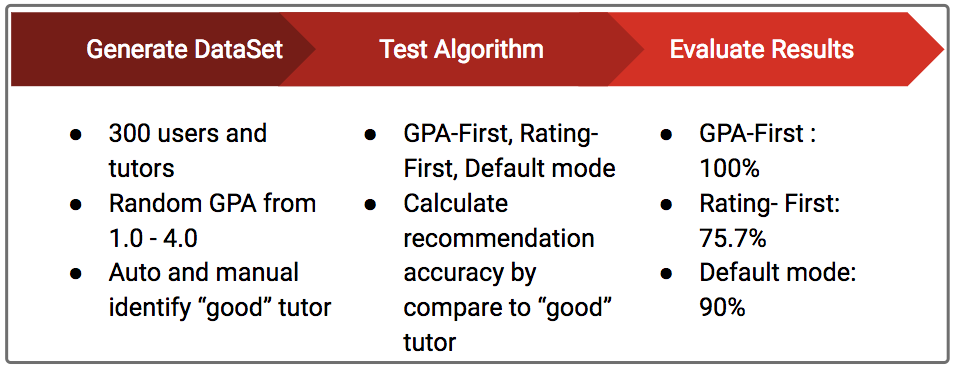
\includegraphics[width=9cm, height=4cm]{algo-evaluation-process.png}
\end{figure}

\paragraph{Generate Dataset}
We need a database which contains a fair mont of user and tutor to work with. 
Manually adding users and tutors through the slack app interface will be too time-consuming. 
Instead, the python script described in section \ref{sec:mock} was used to automatically generate a fixed number of users and tutors, along with their randomly assigned attributes. For the quantitative testing, the most important attributes are the ones related to tutor experience and academic performance - review scores and tutor GPA. These attributes are directly used in the matching and suggestion algorithms.

In this quantitative verification, we used that script to generate 300 users and 300 tutors saved into two separated json file. Each tutor was assigned a random number of reviews with random rating ranged from 1- 5. Each tutor also was assigned a random academic performance - GPA with a number ranged from 1-5. 

\paragraph{Test Design and Excution} 
We designed three major test cases to evaluate the suggestion algorithms. 1) GPA-First: while a user was searching the tutor, they may demand some tutors with high academic performance, here we use GPA as the indicator. In this case, the suggestion algorithms should output a list of tutors which was GPA dominate the order. 2) Rating-First: the same scenario except that user may demand tutors with high tutoring performance, the history rating they got from previous sessions. 3) Default mode: user does not have any preference, but will get a list of suggested tutors with a weighted average score of all kinds of metrics.

We implemented these test cases in Node js, executed along with all other test cases, and saved the recommended lists of tutors of each test cases into JSON files for more quantitive analysis.

\paragraph{Accuracy Result} 
In order to analyze the accuracy of each scenario, we need to define the good tutor sets first. 1) GPA-First: we sorted the tutors by their GPA score, then picked the top 20 as the good tutor set. 2) Rating-First: we sorted the tutors by their average rating, then picked the top 20. 3) Defaut mode: we considered all the tutors with GPA higher than 3.0 and rating higher than 3.0 as the good tutor set.

After we identified the method to extract the good tutor sets, we coded in python script. This script can also do the extraction information from test result JSON file, then computed how many suggested tutors are in the good tutor set, this will be the accuracy for a certain scenario. We ran each scenario for each user and averaged the accuracy as the final results. Figure \ref{fig:algo-evluation-process} show the results.

%%% Local Variables:
%%% mode: latex
%%% TeX-master: "../main"
%%% End:
